\documentclass[14pt]{extarticle}
\usepackage[utf8]{inputenc}
\usepackage{amsmath}
\usepackage{amssymb}
\usepackage[lmargin=1.5in, rmargin=1.5in, bmargin=0.75in]{geometry}
\usepackage{enumitem}
\usepackage{etoc}
\usepackage{fancyhdr}
\usepackage{pgfplots}
\pgfplotsset{compat=newest}
\usepackage{graphicx}
\pagestyle{fancy}
\fancyhf{}
\fancyhead[R]{\thepage}

\renewcommand*\contentsname{Table of Contents}
\renewcommand{\headrulewidth}{0pt}
\graphicspath{ {./img/} }
\setcounter{tocdepth}{1}

\etocsettocstyle{}{}

\begin{document}

\begin{titlepage}
   \begin{center}
       \vspace*{1cm}

       \textbf{\LARGE Analytic Continuity, Gamma, and Zeta Function}

       \vspace{0.5cm}
       {\Large ...and the distribution of primes}
            
       \vspace{1.5cm}

       \textbf{\Large Aditya Diwakar}

       \vfill
            
       \large{A mathematics exploration project for\\
       Complex Analysis
            
       \vspace{0.8cm}
     
       Georgia Institute of Technnology\\
       May 1st, 2021}
            
   \end{center}
\end{titlepage}

\section{Introduction}

Throughout this project, we will take a close look at the inner workings of both the Gamma ($\Gamma$) and Zeta ($\zeta$) functions and their applications to complex analysis. 

Both of these functions are critical to various fields and are related to each other by the principle of analytic continuation. This begs the following questions:
\begin{enumerate}[label=(\arabic*)]
	\item What is the Gamma function? What does it mean? How does it relate to complex analysis?
	\item What is the Zeta function? What interesting properties does it have relating to other fields?
 	\item What is analytic continuation? How is this related to the previous questions?
\end{enumerate}

\noindent
This project will thoroughly explain each of the aformentioned questions and go into detail
about the connections to complex analysis. The ordering of this project will appear 
unintuitive at first, but is helpful when attempting to connect topics together. 

\tableofcontents
\pagebreak
\setcounter{tocdepth}{3}

\section{Riemann's Zeta Function}
\localtableofcontents

\vspace{1cm}
\noindent
If you have ever been interested in mathematical myseteries, you most likely have heard of the
zeta function. It is given the name \textit{Riemann Zeta Function} as it was a powerful extension
of Euler's earlier work studied by Bernhard Riemann, the \textit{``father"} of complex analysis.

We start with a definition. The Zeta function is defined simply as an infinite series:
\begin{align*}
	\zeta(s) = \sum_{n=1}^{\infty} \left(\frac{1}{n}\right)^ = \frac{1}{1} + \frac{1}{2^2} + 
	\frac{1}{3^s} + \cdots
\end{align*}

It is, trivially, well defined for any value of $s \in (1, \infty] \subset \mathbb{R}$. But,
there are powerful extensions of this function into a larger region. We first take a few examples,
let us say $s = 2$ and evalute $\zeta(s)$ which is simply:
\begin{align*}
	\zeta(2) = \sum_{n=1}^{\infty} \left(\frac{1}{n^2}\right) = \frac{1}{1} + \frac{1}{4} + 
	\frac{1}{9} + \frac{1}{16} + \cdots
\end{align*}
It is clear that this computation obviously converges, but the result is not as obvious. In fact,
this specific example highlights the utility of the zeta function, as (surprisingly) $\zeta(2) = \pi^2 / 6$. There are numerous examples of interesting phenomenon when $s > 1$ that are worth
exploring, but $s \leq 1$ is where this function relates to complex analysis and is what we will
cover.

\subsection{Divergence of Zeta}
Let us note the result when $s \leq 1$. First, let us take $s = 1$ and notice $\zeta(s)$ will
simply become the harmonic series. In fact, take any number $s \leq 1$ and it immediately
follows that $\zeta$ diverges. In fact, let us take $s = -1$ and see that
\begin{align}
	\zeta(-1) = \sum_{n = 0}^{\infty} \left(\frac{1}{n}\right)^{-1}	= \sum_{n = 0}^{\infty} n = 1 + 2 + 3 + \cdots \label{neg_zeta}
\end{align}
which obviously diverges. This begs the question, why are we even talking about it? It must
be that this function is useless out of the previously mentioned domain. Wrong!

\subsection{Filling It In}
Up to this point, we have discussed that the $\zeta$ is useless outside of the domain it converges in. In fact, there is truth to this! The \textit{traditional} definition becomes useless as
\begin{align*}
	\zeta(s) = \sum_{n = 0}^{\infty} \left(\frac{1}{n}\right)^s
\end{align*}
will never give converging values out of this domain. However, there is merit to extending
this domain.

\begin{center}
	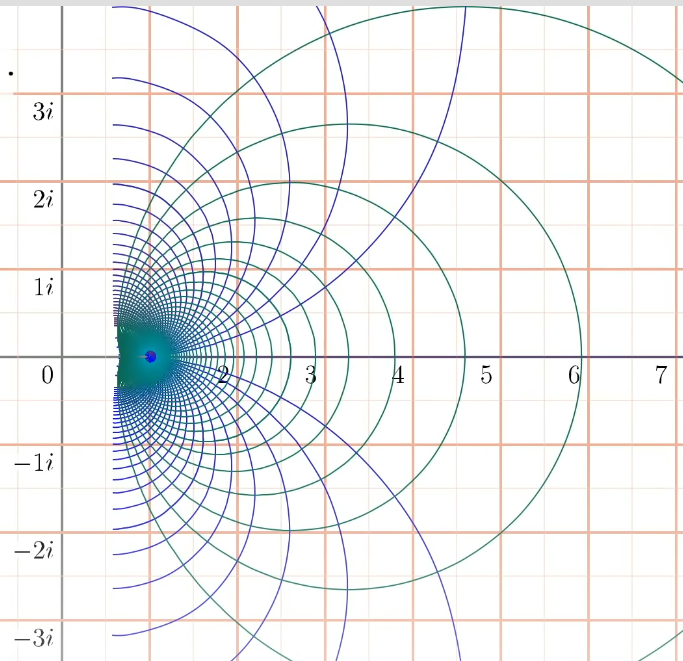
\includegraphics[scale=0.3]{zeta_undeveloped}
\end{center}
This image (which is the value from the zeta function when inputs are $s > 1$ is begging for an 
extension. By inspection, it looks incomplete even though these are all the valid outputs
considering the input field.

Also, it was left off that $\zeta$ is capable of handling complex inputs, but $\Re(z) > 1$
still. This is by virtue of how complex exponents work, a topic discussed in elementary
complex analysis.

In order to extend this function, we can simply pick and choose values for other inputs. For
example, if we agreed to set $\zeta(-1) = \frac{-1}{12}$ (see equation (\ref{neg_zeta})), then we have one value in the 
undetermined domain. We can continue doing this and there would be an infinite number of
possibilities for what this function can be. In other words:
\begin{align*}
	\zeta(s) = \begin{cases}
		\sum_{n = 0}^{\infty} \left(\frac{1}{n}\right)^s & \Re(s) > 1\\
		\text{anything else} & \Re(s) \leq 1
	\end{cases}
\end{align*}

\subsection{Analytic Continuation}
From the previous section, we noted that we can have an infnite number of possible extended $\zeta$ functions that take into account
$\Re(s) \leq 1$. However, there is only one that is uniquely determined if we had one restriction. So, what is that restriction?

Let us say that the extension of $\zeta$ had to be analytic everywhere, just as $\zeta$ is when $\Re(s) > 1$. In other words and more
simplified words, this must mean that the angles from the pre-image are preserved when mapped to the image by $\zeta$.

If we require this, then we get a uniquely determined extension that looks like:
\begin{center}
	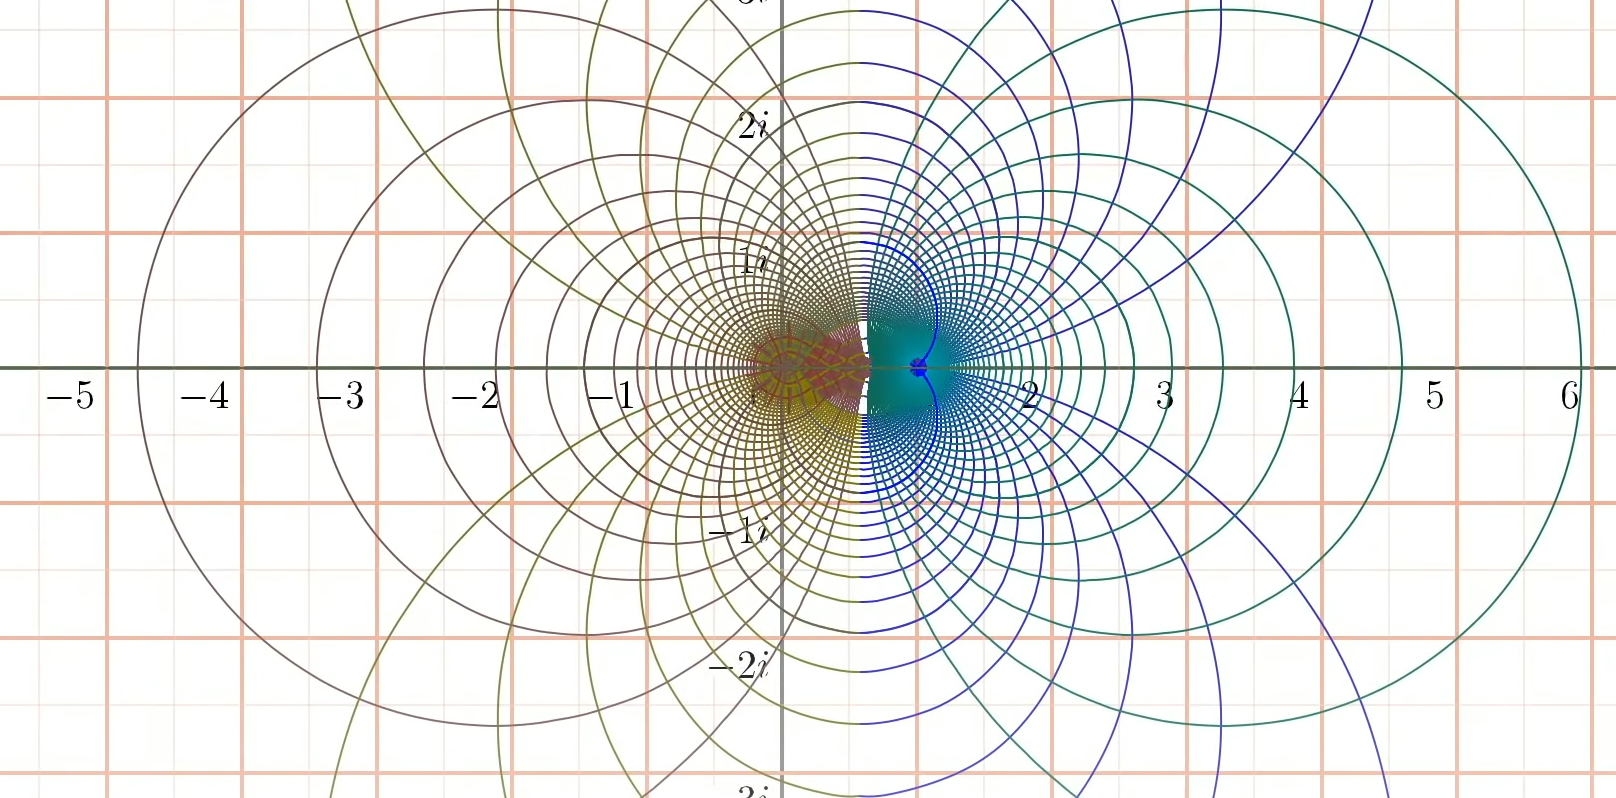
\includegraphics[scale=0.225]{zeta_developed}
\end{center}

The important aspects of the graph from above is that there is a symmetry. This is a result of how the unqiuely determined analytic
extension requires there to be a derivative everywhere. In other words, this must satisfy the \textit{Cauchy Riemann} equations.
\begin{align*}
    \frac{\partial u}{\partial x} = \frac{\partial v}{\partial y} \quad\quad\quad
    \frac{\partial u}{\partial y} = -\frac{\partial v}{\partial x}
\end{align*}

\subsection{Consequences}
With an extension of the $\zeta$ function created using an \textit{analytic continuation}, we should point out some of the consequences.

In this uniquely determined analytic continuation, the value of equation (\ref{neg_zeta}) is $\frac{-1}{12}$. In other words:
\begin{align*}
    \sum_{n = 0}^{\infty} n = \sum_{n=0}^{\infty} \left(\frac{1}{n}\right)^{-1} = \zeta(-1) = \boxed{-\frac{1}{12}}
\end{align*}
This brings rise to the popular misconception that the infinite series (which clearly diverges in a traditional sense) is:
\begin{align*}
    1 + 2 + 3 + 4 + \cdots = -\frac{1}{12}
\end{align*}
There is merit to this intepretation of giving infiite diverging series a finite value, but that is out of the scope of this paper.

Another example of this phenomenon is when $\zeta$ is evaluated at $s = 0$. When $s = 0$, we have:
\begin{align*}
    \zeta(0) = \sum_{n = 0}^{\infty} \left(\frac{1}{n^0}\right) = \sum_{n = 0}^{\infty} 1 = 1 + 1 + 1 + \cdots = -\frac{1}{2}
\end{align*}
In other ways, the $\zeta$ functio says that the infinite sum of $1 + 1 + 1 + \cdots$ is equal to $-\frac{1}{2}$ which intuitively makes sense.

\subsection{Coming Up...}
The mysteries of this function are not limited. The zeta function has an important relationship to prime numbers that will be explained in
another section. 

However, the important takeaways from this section is the power of analytic continuation and how it can be used to 
expand the domain of a function onto another (potentially more useful) region.

\pagebreak

\section{Gamma Function}
\localtableofcontents

\vspace{1cm}
\noindent
Advanced mathematical scholars may know of a gamma function defined as:
\begin{align*}
    \Gamma (n) = (n - 1)!
\end{align*}
which has an alternative definition given by:
\begin{align*}
    \Gamma(z) = \int_0^\infty x^{z - 1} e^{-x} dx
\end{align*}
when $\Re(z) > 0$. Similar to the zeta function, this function has no values when $Re(z) < 0$. The gamma function is generally intended to
be only used for positive integers. After all, the initial definition of $\Gamma(n) = (n - 1)!$ makes no room for non-positive non-integer
inputs in the domain.

However, our alternative definition over the complex plane allows a much more versatile usage that is not limited to simply positive integers.
Rather, it is only limited to complex numbers with positive real components. 

\subsection{Usage of Extended Definition}

Let us take the first and most common example of the extended gamma function definition, when $z = \frac{1}{2}$. In which case, we have:
\begin{align*}
    \Gamma\left(\frac{1}{2}\right) = \int_0^\infty x^{-1/2} e^{-x} dx  = \sqrt{\pi}
\end{align*}

Since $\Gamma(n) = (n-1)!$, this integral yields a very important result and an even more important conclusion:
\begin{align*}
    \Gamma(1/2) = \sqrt{\pi}
    \implies \left(\frac{1}{2} - 1\right)! = \left(-\frac{1}{2}\right)! = \sqrt{\pi}
\end{align*}

In essence, this extended definition gives new meaning to an otherwise arbitrary concept (factorial of negative numbers and fractions).

\subsection{Analytic Continuation}
It should be clear here that we have already defined our analytic continuation. In this case, our original function was $\Gamma(n) = 
(n-1)!$ which has a domain of $n\in \mathbb{Z} \setminus \{0\}$ to a function that has a significantly larger domain $\forall z\in
\mathbb{C}$ with a restriction that $\Re(z) > 0$.

However, the extended analytically continued gamma function defines an iterative property such that any integer fraction can be part
of the domain which extends the pre-image of the function by significantly more. 

\begin{center}
	\begin{tikzpicture}[scale=1.2]

	\begin{axis}[
	xmin = -4.9, xmax = 5.1, 
	%ymin = -3.5, ymax = 3.5,  
	restrict y to domain=-6:6,
	axis lines = middle,
	axis line style={-latex},  
	xlabel={$x$}, 
	ylabel={$y$},
	%enlarge x limits={upper={val=0.2}},
	enlarge y limits=0.05,
	x label style={at={(ticklabel* cs:1.00)}, inner sep=5pt, anchor=north},
	y label style={at={(ticklabel* cs:1.00)}, inner sep=2pt, anchor=south east},
	]

	\addplot[color=red, samples=222, smooth, 
	domain = 0:5] gnuplot{gamma(x)};

	\foreach[evaluate={\N=\n-1}] \n in {0,...,-5}{%
	\addplot[color=red, samples=555, smooth,  
	domain = \n:\N] gnuplot{gamma(x)};
	%
	\addplot [domain=-6:6, samples=2, densely dashed, thin] (\N, x);
	}%
	\end{axis}
	\end{tikzpicture}
\end{center}

\subsection{Gamma and Poles}
An interesting side effect of the gamma function is by virtue of yet another definition that points out the poles of $\Gamma$. As we are
interested more in the consequence and less about the direct proof, we can assume that the definition for $\Gamma$ is true and is given 
by an iteratve formula, like so:
\begin{align*}
    \Gamma(z) = \frac{\Gamma(z + n + 1}{z(z + 1)(z + 2)\cdots(z + n)}
\end{align*}
Obviously, this has poles at $z = 0, 1, 2, \ldots, n$. By virtue of this equation, we have a very simple equation for the residues
of these simple poles (poles with order $1$), this is given by:
\begin{align*}
    \underset{z = z_0}{\mathrm{Res}} f(z) = \frac{(-1)^n}{n!}
\end{align*}
From this, we can solve for the residues of $z = 0, 1, 2, 3, \cdots, n$. They are given by:
\begin{align*}
    \underset{z = 0}{\mathrm{Res}} f(z) = 1 \quad
    \underset{z = 1}{\mathrm{Res}} f(z) = -1\quad
    \underset{z = 2}{\mathrm{Res}} f(z) = 2\quad\\[2mm]
    \underset{z = 3}{\mathrm{Res}} f(z) = -6\quad
    \underset{z = 4}{\mathrm{Res}} f(z) = 24\quad
    \underset{z = 5}{\mathrm{Res}} f(z) = -120\\
\end{align*}

\subsubsection{Visualization of $|\Gamma(z)|$}

Notice that a graph of these residues would be exponentially decreasing (inverse factorial) and so an image of the norm of the $\Gamma$
function could visually be:
\begin{center}
    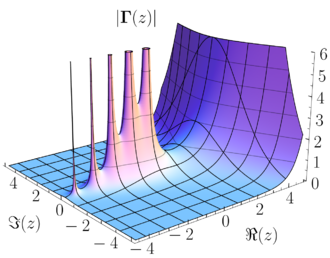
\includegraphics[scale=0.75]{gamma_poles}
\end{center}

Identify in this graph that as we travel down $\Im(z) = 0$ and as $\Re(z) \to \infty$ with $z\in \mathbb{Z}$, there are \textit{``spikes"}
that get progressively thinner. This is due to the previously mentioned principle of their residues decreasing exponentially.
\pagebreak

\section{Exploration: Distribution of Primes}

\pagebreak

\section{Problems}

\pagebreak

\section{Conclusion}

\end{document}

